\documentclass{elteikthesis}

\usepackage{url}
\usepackage{fancyhdr}
\usepackage{indentfirst}
\usepackage{ucs}
\usepackage[utf8]{inputenc}
\usepackage[T1]{fontenc}
\usepackage[english,hungarian]{babel}
\selectlanguage{hungarian}

\title{Rendezési algoritmusok szemléltetése}
\author{Márföldi Péter Bence}
\supervisor{Veszprémi Anna}
\supervisorstitle{mestertanár}
\period{programtervező informatikus BSc}
\thesisyear{2015}
\department{Algoritmusok és Alkalmazásaik Tanszék}

\fancyhf{}
\fancyhead[L]{\rightmark}


\begin{document}

\frontmatter

	\maketitle
	\tableofcontents
	
\mainmatter

	\cfoot{\thepage}
	\pagestyle{fancy} 

\chapter{Bevezetés} 
Az bizonyos, hogy minden informatikus - beleértve a leendőeket is - tanulmányaik kezdetén találkoztak a rendezési algoritmusokkal. Nagyszerű terület arra, hogy megérthessük a műveletigény kérdését, azt hogy mi számít igazán sok adatnak, vagy éppen, hogy mit értünk egy algoritmus stabilitásán.

\section{A feladat és annak értelmezése} 
\section{Definíciók és jelölések}
\subsection{Oszd meg és uralkodj elv}
Egy algoritmus tervezési stratégia. Az elv\cite{Cormen} a következőképp old meg egy problémát:
\begin{description}[0.5cm]
	\item[$\bullet$] Az eredeti problémát felosztja kisebb az eredetihez hasonló típusú feladatokra.
	\item[$\bullet$] Rekurzívan megoldja ezeket a kisebb problémákat.
	\item[$\bullet$] A kisebb részek megoldásait összevonva,  megoldást ad az eredeti feladatra.
\end{description}


\section{Alkalmazott technológiák}
A Következőkben röviden összefoglaljuk a Java\cite{Java} és a JavaFX\cite{JavaFX} jellegzetességeit.
\subsection{A Java-ról röviden}
A Java egy általános célú, objektumorientált programozási nyelv, melyet 2009-ig a \emph{Sun Microsystems} fejlesztett, ezt követően pedig az \emph{Oracle}. A szakdolgozatban használt 1.8-as verziót már az \emph{Oracle} adta ki 2014-ben. A Java nyelv a szintaxisát a C és C++ nyelvektől örökölte, azonban utóbbitól eltérően egyszerű objektummodellel rendelkezik. \par
 A Java platformra készült programok túlnyomó többsége asztali alkalmazás. Manapság egyre több helyen találkozhatunk a Java nyelven írt programokkal, például mobil eszközökön, banki rendszereknél vagy akár egy szórakoztató elektronikai eszközön. Nagy előnye, hogy sok nyelvvel ellentétben platformfüggetlen, azaz egy adott platformról egy program minimális változtatással átültethető egy másik platformra. \par
 A Java legfontosabb része a \emph{Java virtuális gép (JVM)}. A \emph{JVM}-et sokféle berendezés és szoftvercsomag tartalmazza, így a nyelv egyaránt platformként és középszintként is működik.
Összefoglalva a Java program három fontos szerepet tölt be:
\begin{description}[0.5cm]
\item[$\bullet$] programozási nyelv
\item[$\bullet$] köztes réteg (middleware)
\item[$\bullet$] platform
\end{description}

\subsection{JavaFX}
Olyan szoftverplatform, amelynek célja, hogy gazdag internetes alkalmazást lehessen készíteni és futtatni eszközök széles skáláján. Eredetileg a \emph{Swing} könyvtárat váltotta volna fel, azonban jelenleg mindkettő része a \emph{Jave SE}-nek. \par
 A 2.0-ás verzióig a fejlesztők egy külön nyelvet használtak, amelyet \emph{JavaFX Script}-nek neveznek. Azonban mivel ez szintén Java bájtkódot generál a későbbiekben megadatott a lehetőség, hogy a programozók Java kódot használjanak helyette. A JavaFX egyik legnagyobb előnye, hogy egy egyszerű \emph{XML} struktúrában leírhatók a program grafikus felületének összetevői, melyhez ezt követően elegendő az egyes interakciókhoz tartozó funkciókat implementálni.\par Az elterjedtebb operációs rendszerek mindegyikét támogatja. Ahogyan előnye, úgy hátránya is a \emph{Swing}-hez képest az, hogy jelenleg is folyik a fejlesztése, ezért olykor csak hosszas utánajárást követően sikerül megoldást találni egy-egy problémára.

\chapter{Felhasználói dokumentáció}

\section{A vizsgált algoritmusok}

\subsection{Buborékrendezés}
A legrégebbi és a legegyszerűbb rendezési algoritmus. Mindemellett a legtöbb esetben a leglassabb is. Már az 1965-ös évben megjelent egy teljes körű elemzése\cite{Demuth}.\par
 A rendezés minden egyes elemet összehasonlít a rákövetkező elemmel, és ha szükséges megcseréli őket. Mindezt addig, amíg nincs egy olyan menet, amelyben egyetlen elem sem cserél helyet. Ez azt eredményezi, hogy lépésenként a maximális elem "buborék" szerűen a lista végére kerül, ezzel egyidejűleg a kisebb elemek "lesüllyednek" a tömb elejére. Az algoritmus javítható azzal, hogy nem vizsgáljuk meg minden menetben a tömb összes elemét, hanem amennyiben egy maximális elem elérte a helyét visszavezetjük a problémát az eggyel "rövidebb" rendezési feladatra\cite{Fekete}.

\subsection{Beszúró rendezés}
A nevéből egyszerűen kikövetkeztethető az eljárás: beszúrja az elemeket a megfelelő helyükre a végleges tömbbe. Lényege, hogy a soron következő elemet egy ideiglenes változóba mentjük, és a rendezett tömb elemeit jobbra csúsztatjuk, mindaddig amíg a kiválasztott érték nem kerül a helyére. Kezdetben a tömb első elemét tekintjük rendezettnek. A legtöbb esetben akár kétszer hatékonyabb a Buborékrendezéshez képest.\cite{Fekete} Továbbá kis (néhány száz) elemszámú bemenetre az egyik leghatékonyabb algoritmus.

\subsection{Shell rendezés}
Donald Shell nevéhez fűződik, a legtöbb esetben a leggyorsabb négyzetes idejű algoritmus. Többször vizsgálja a tömböt, és minden alkalommal egy részén beszúró rendezést hajt végre. Arra, hogy mekkora méretű résztömböt vizsgáljon az egyes lépésekben az algoritmus több javaslat is található. Az algoritmus nevét is adó Donald Shell $\lfloor N/2^k \rfloor$ (k>=1) lépésközt javasol. Azonban így az algoritmus időkomplexitása legrosszabb esetben $\Theta(N^2)$. Az algoritmus sebessége nagyban függ a lépésköz megválasztásától.

\subsection{Gyorsrendezés}
C.A.R. Hoare\cite{Horae} alkotta meg 1965-ben. Az egyik leggyorsabb rendezési eljárás, ezért rendkívül gyakran alkalmazzák.\par
Helyben rendező, oszd meg és uralkodj\cite{Cormen} elven működő rekurzív algoritmus. A következő négy lépésre bontható fel az rendezés:
\begin{description}[0.5cm]
	\item[$\bullet$] Ha csak egy vagy nulla elemű az elemzett rész, akkor ne tegyünk semmit.
	\item[$\bullet$] Válasszunk egy vezérelemet (legjobb oldalibb elem).
	\item[$\bullet$] A rendezendő részt vágjuk ketté, az egyik oldalára a vezérelemtől kisebb, míg a másikra a nagyobb elemek kerüljenek.
	\item[$\bullet$] Rekurzívan ismételjük meg az előbbi lépéseket a résztömbökön.
\end{description}
A rendezés műveletigényét befolyásolja, hogy hogyan választjuk meg a vezérelemet. Például a legnagyobb műveletigényt ($\mathcal{O}(n^2)$) eredményezi, ha mindig a legjobboldalibb elemet választjuk vezérelemnek, és a tömb elemei csökkenő sorrendben vannak. Éppen ezért a gyakorlatban javasolt ezen elem véletlenszerű megválasztása. A gyorsrendezés a legtöbb esetben(közepes és nagy méretű bemenetre) a legjobb választás ha számít a rendezés sebessége. Azonban ha a tömb elemei már eleve rendezettek vagy esetleg fordított sorrendben szerepelnek sajnos nem hatékony. Ezekben az esetekben ajánlatos másik algoritmust használni. 

\subsection{Versenyrendezés}
A maximum-kiválasztó rendezések közé tartozik, minden egyes menetben kiválasztja a legnagyobb elemet, kiírja és végül eltávolítja. A maximum kiválasztásnak a gyakorlati hátterét a sportesemények lebonyolítási rendje adja, azaz meghatározza az elemek között a "nyertest". A módszert n=2$^k$ inputhossz esetén érdemes alkalmazni, mivel ettől értérő bemenetre sokkal kedvezőbb eredményt lehet elérni a kupacrendezéssel. Az algoritmus által használt adatszerkezet egy teljes bináris fa.

\chapter{Fejlesztői dokumentáció}

\section{Tervezés és megvalósítás}
A fejlesztés során több szempontot is figyelembe kell venni, úgy mint: műveletigény, memóriaigény, jó megjelenés, egyszerű kezelhetőség, és átlátható-, bővíthető kód készítése. Mivel ezen kritériumok közül több is csak egy másik rovására javítható, ezért a tervezés során kompromisszumokat kell kötni. Továbbá fel kell készülni arra, hogy az eredeti terven a fejlesztés során módosításokat kell végezni, mivel egy-egy probléma megoldása más megközelítést kívánhat.

\subsection{Tervezés}
A dolgozat fő célja egy olyan elsősorban hallgatóknak szánt program létrehozása, amellyel néhány rendezési algoritmus működése egy letisztult és egyszerű felhasználó felületen keresztül tanulmányozható.\par
A programnak három jól elkülönülő részből kell állnia:
Egy logikai(modell) részből, ami gyakorlatilag a rendszer "motorja", itt kell, hogy történjen mindenféle számítási és adattárolási művelet. Egy megjelenítési rétegből, amely a logikai rész eredményeit jeleníti meg a felhasználó számára. Végül pedig egy kontroller szintből, amely kapcsolatot teremt a logikai- és a megjelenítési réteg között. A gyakorlatban ezt a fajta tagolást nevezik Modell-Nézet-Vezérlő \emph{(MVC)} tervezési mintának.

\subsection{Megvalósítás}
Az első lépés a rendezési algoritmusok implementálása.
Ezt követhette egyszerűbb felhasználói felület létrehozása. Kezdetben elegendő, ha csak egy grafikon jelenik meg, amely reprezentálja a tömbben található számokat.\par
\begin{figure}
	\centering
	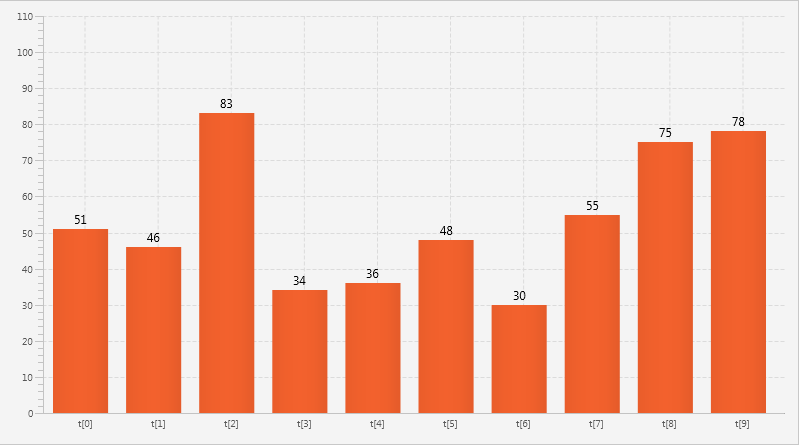
\includegraphics[width=0.5\textwidth]{pics/diagram.png}
	\caption{A tömb megjelenítése egy oszlopdiagramon}
\end{figure}
Két algoritmushoz szükséges a gráfos reprezentáició, így a következő lépés egy gráf implementálása.
Ezt követően a cél, hogy néhány "beégetett" elemre a rendezések lejátszhatóak legyenek, és az aktuális állapota a tömbnek szinkronban legyen a diagrammal valamin a gráffal. Később az egyes lépésekben történő összehasonlításokat/vizsgálatokat, mozgatásokat, cseréket kell különböző színekkel jelölni a diagramon és számon tartani ezen műveletek összegeit.\par
Ezen a ponton az módosítás történt a projekt tervein. Eredetileg egy-egy külön szálon futottak volna az algoritmusok, és a felhasználói interakció hatására ezek állapota változott volna. Azonban a \emph{JavaFX} szálkezelése jelentősen eltér az szokványos szálkezelésétől, ezért járhatóbb útnak bizonyult az, hogy kétszer kerüljenek implementálásra az algoritmusok. Az egyik implementációban számon tartjuk az éppen aktuális állapotot, és ez jelenik meg a felhasználói felületen. A másik megvalósításban pedig az algoritmusok azonnal lejátszódnak, így képet kaphatunk arról, hogy mennyi műveletre volt szükség a rendezés során. Ezen utóbbi implementációk mindegyike külön szálon fut, és ahogy valamelyik befejeződik figyelmezteti a főprogramszálat, hogy jelenítse meg a műveletek számát.\par
Miután a program alapjai elkészültek kezdetét veheti a a felhasználói felület részletes kialakítása. Elsőként a diagram elhelyezése egy panelen, amely tartalmaz továbbá egy listát a választható algoritmusokról.\par
A programnak egy fontos szolgáltatása az, hogy a felhasználó különböző adatbeviteli mód közül választhat. A logikai réteget ki kell bővíteni ezekkel az esetekkel, továbbá a felhasználói felületen lehetőséget adni ezen módok kiválasztására.\par
Ezután az eszköztár kerül a helyére, mellyel párhuzamosan megtörténik az egyes műveletekhez tartozó eljárások implementálása.\par
Végül a rendezések összehasonlítására lehetőséget adó panel létrehozása, egy táblázattal, benne az algoritmusok műveletigényével. Továbbá egy diagrammal, amin megjelenik a táblázatból kiválasztott sor összehasonlításainak és mozgatásainak a száma.


\subsection{Használt fejlesztőeszközök}
A fejlesztés \emph{Eclipse SDK 4.4} fejlesztői környezet keretei között történt. A program grafikus fejlesztői felületet ad alkalmazások készítéséhez.\par
A program elkészítése során a kódolást segítő funkció volt a kódkiegészítés, továbbá az egyik beépített projektmenedzsment eszköz(\emph{EGit}). Az egész projekt megtalálható, és az egyes verziói visszakövethetők a GitHub-on: \url{https://github.com/marfoldi/SRTNLGRTHMS}\par
A fejlesztéshez elengedhetetlen a \emph{Java SE 8u40} vagy magasabb verziójú szoftver. Továbbá a fejlesztést nagyban elősegítette a \emph{JavaFX Scene Builder 2.0}, melynek segítségével egyszerűen megtervezhetővé váltak a grafikus felület komponensei.\par
A program fejlesztése során nem került sor külső függvénykönyvtár használatára.
\begin{thebibliography}{widest entry}
\bibitem{Java}
\emph{Java (programming language)},
Wikipedia the free encyclopedia.
[ONLINE] [Hivatkozva: 2015.04.21]
\url{http://en.wikipedia.org/wiki/Java_(programming_language)/}
\bibitem{JavaFX}
\emph{JavaFX},
Wikipedia the free encyclopedia.
[ONLINE] [Hivatkozva: 2015.04.21]
\url{http://en.wikipedia.org/wiki/JavaFX/}
\bibitem{Demuth}
Demuth, H.:
\emph{Electronic Data Sorting},
PhD thesis, Stanford University,
1956, [184]
\bibitem{Fekete}
Dr. Fekete István:
\emph{Algoritmusok és adatszerkezetek I. jegyzet},
[ONLINE] [Hivatkozva: 2015.04.20] \url{http://people.inf.elte.hu/fekete/algoritmusok_bsc/alg_1_jegyzet/}
\bibitem{Cormen}
Thomas H. Cormen, Charles E. Leiserson,Ronald L. Rivest, Clifford Stein:
\emph{Új algoritmusok},
Scolar kiadó, 2003,
[992], 9789639193901
\bibitem{Horae}
C.A.R. Hoare:
\emph{Algorithm 64: Quicksort}
Communications of the ACM, 4, 7, 1961
[321]
\end{thebibliography}

\end{document}